%----------------------------------------------------------------------------------------
%	SOLUTION 1.a
%----------------------------------------------------------------------------------------
\subsection*{Solution 1.a}
Fig.~\ref{fig:q1_a} shows the decision boundary for the dummy data created in Q1.a. The error rate on this dataset is $0\%$.
\begin{figure}[h!]
	\centering
	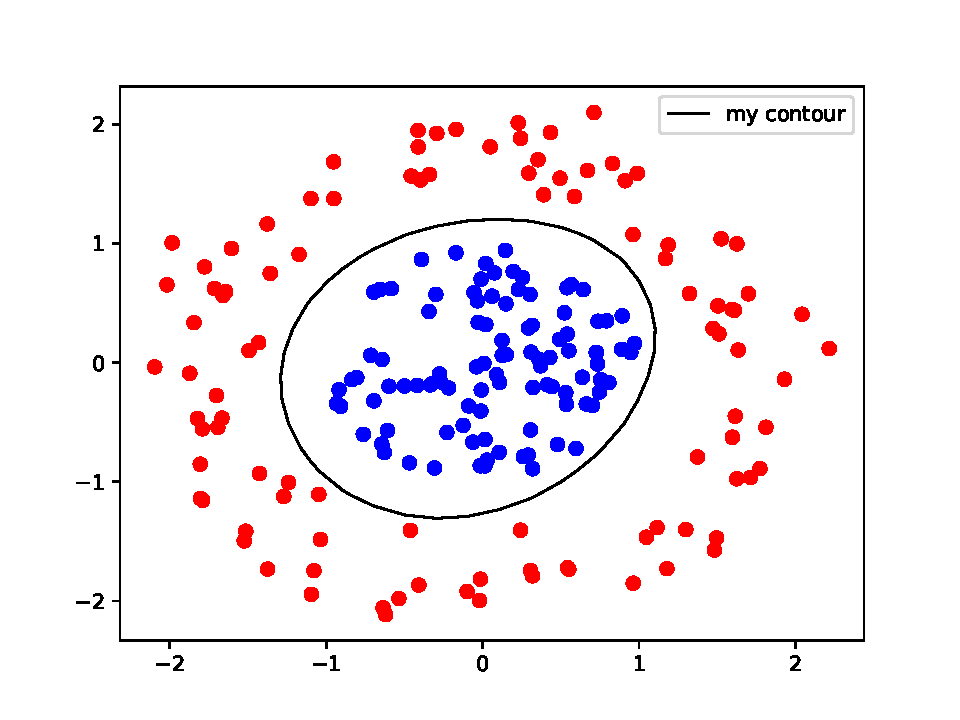
\includegraphics[scale=0.5]{q1_a_my_contour.pdf}
	\caption{Classification with polynomial kernel of degree $3$}
	\label{fig:q1_a}
\end{figure}
%----------------------------------------------------------------------------------------
%	SOLUTION 1.b
%----------------------------------------------------------------------------------------
\subsection*{Solution 1.b}
Fig.~\ref{fig:q1_b} shows the decision boundary returned by 'svc' function of 'SVM' module of 'sklearn' package with the same kernel as previous one.
\begin{figure}[h!]
	\centering
	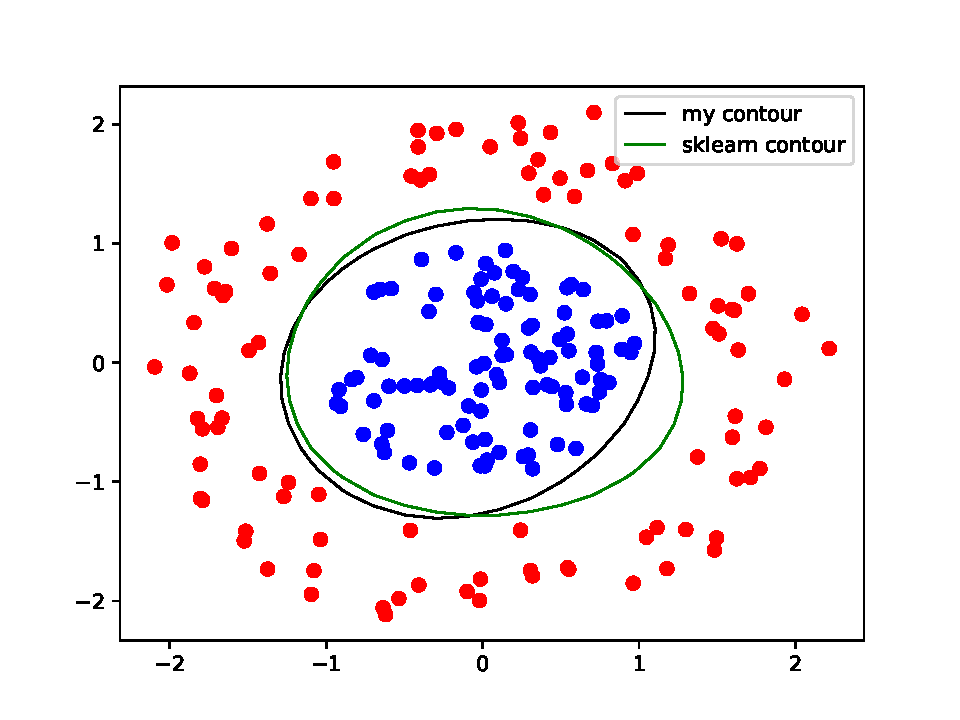
\includegraphics[scale=0.5]{q1_a_svc_contour.pdf}
	\caption{Classification with polynomial kernel of degree $3$ with scikit-learn module}
	\label{fig:q1_b}
\end{figure}
Fig.~\ref{fig:q1_b} shows that the decision boundary returned by 'sklearn' is better because of the additional regularization parameter used by 'sklearn' package. Fig.~\ref{fig:q1_b} shows the decision boundary for regularization parameter $C = 0.05$.
\begin{figure}[h!]
	\centering
	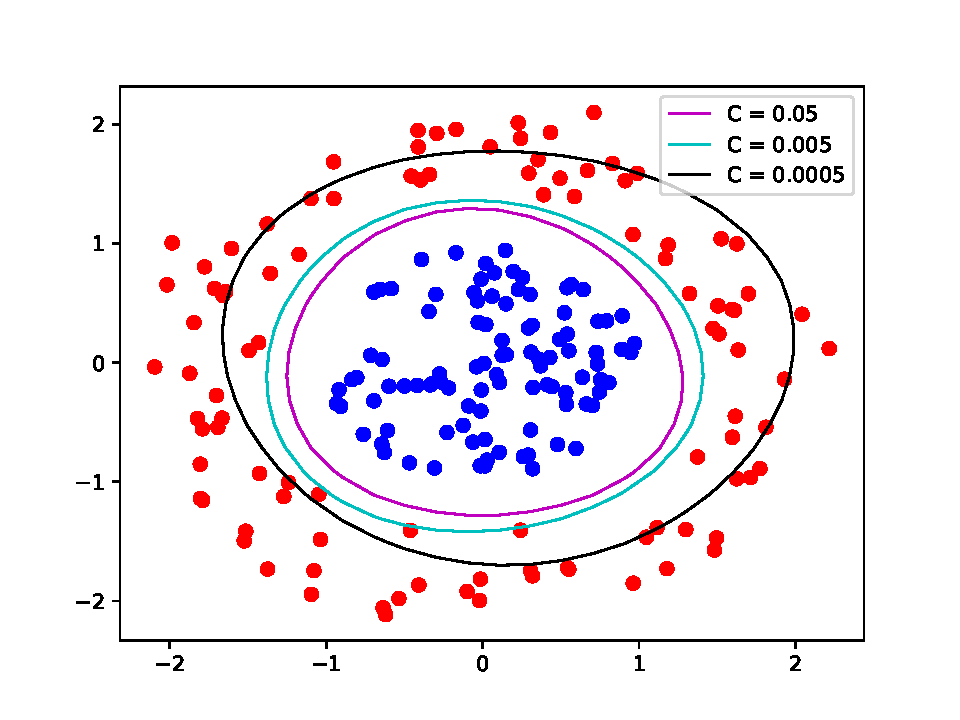
\includegraphics[scale=0.5]{q1_a_svc_c_effect.pdf}
	\caption{Classification with polynomial kernel of degree $3$ with different regularization parameter $C$ of scikit-learn module}
	\label{fig:q1_b1}
\end{figure}
Fig.~\ref{fig:q1_b1} shows that decreasing the regularization parameter makes the decision boundary wider thus causing more error on training set. On the other hand, increasing the regularization parameter shrinks the decision boundary and too much increment will also cause larger training error.
%----------------------------------------------------------------------------------------
%	SOLUTION 1.c
%----------------------------------------------------------------------------------------
\subsection*{Solution 1.c}
The following table shows the training and test error rates on both 'optdigits49' and 'optdigits79' dataset.
\begin{table}[h!]
	\begin{center}
		\begin{tabular}{||c | c | c ||} 
			\hline
			Dataset & Training error (\%) & Test error (\%)\\ [0.5ex] 
			\hline\hline
			optdigits49 & 0.473 & 3.169\\ [0.5ex]
			\hline
			optdigits79 & 0.355 & 0.709\\ [1ex]
			\hline
		\end{tabular}
	\end{center}
	\caption{Q1.c: Error-rate on subset of optdigit dataset}
\end{table}